\chapter*{2 Versuchsdurchführung und Auswertung}
\addcontentsline{toc}{chapter}{2 Versuchsdurchführung und Auswertung}
\setcounter{chapter}{2}
\setcounter{section}{0}
\setcounter{subsection}{0}

\section{Versuch 1: Frequenz und Dämpfung der freien Schwingung}

    \subsection{Versuchsaufbau und -durchführung}

    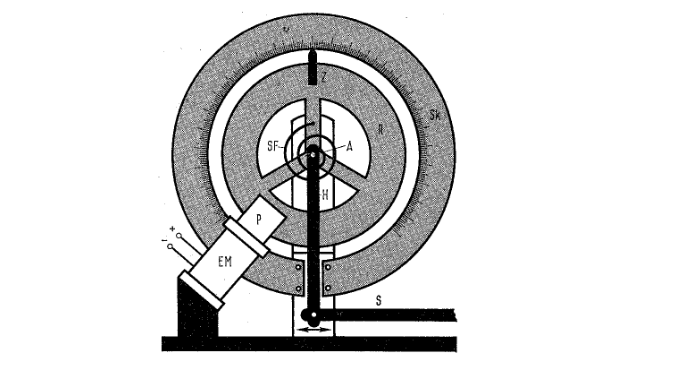
\includegraphics[width=\textwidth]{bilder/Aufbau.png}
    \label{fig:Aufbau1}
    Das Drehpendel in \ref{fig:Aufbau1} besteht aus einer horizontalen Achse (A) einem darum 
    drehenden Kupferring (R), der über eine Spiralfeder (SF) mit einem Hebel (H) verbunden ist und über eine Stange (S) in Bewegung versetzt werden kann.
    Die Amplitude kann an einer festen Skala (Sk) abgelesen werden.

    
    \subsubsection{Teil 1: Eigenfrequenz}
    Der Aufbau ist in \ref{fig:Aufbau1} zu sehen. Die Schwingungsdauer wird mit einer Stoppuhr gemessen. Die Messung wird 5 mal wiederholt und läuft über 10 Perioden.
    Die Messergebnisse sind in Tabelle \ref{tab:Eigenfrequenz} zu sehen.

    \begin{table}[H]
        \centering
        \label{tab:Eigenfrequenz}
        \caption{Messergebnisse Eigenfrequenz}
        \begin{tabular}{|l|l|l|l|l|l|}
            \hline
            Messung \# & 1 & 2 & 3 & 4 & 5\\
            \hline
            $t[s]$ & & & & & \\
            \hline
        \end{tabular}
    \end{table}    

    \subsubsection{Ergebnisse \& Diskussion}
    Man erhält für die 5 Messungen einen Mittelwert für die Periodendauer von TODO. Wir nehmen nun TODO als Messefehler, da Begründung TODO.
    %Der Messfehler lässt sich auf die Reaktionszeit des Menschen zurückführen und darauf das die Stoppuhr 2 mal betägtigt werden muss.
    Da wir über 10 Perioden messen, teilen wir den Messwert durch 10. So erhalten wir den Fehler für eine Periode. Damit ergibt sich nun einen mittlere Periodendauer von DAUER $\pm$ FEHLER.
    Die Frequenz können wir nun mit folgender Formel berechnen:

    \begin{equation}
        \label{eq:Frequenz}
        f = \frac{1}{T}
    \end{equation}
    Daraus resultiert eine Eigenfrequenz von:
    \begin{equation}
        \label{eq:Eigenfrequenz}
        \omega_0 = 2\pi \cdot f = 2\pi \cdot \frac{1}{T} = TODO
    \end{equation}

    Nun können wir noch den geforderten Größtfehler $\Delta \omega_0$ berechnen. Dazu verwenden wir folgende Formel:
    \begin{equation}
        \label{eq:Größtfehler}
        \begin{aligned}
        \Delta f &= f \cdot \frac{\Delta T}{T} \\
        \Delta \omega_0 &= \left|2\pi \cdot -\frac{1}{T^2} \cdot \Delta T\right|
        \end{aligned}
    \end{equation}

    TODO Diskussion?
        \subsubsection{Teil 2: Dämpfung}
        Der Versuchsaufbau ist auch hier in \ref{fig:Aufbau1} zu sehen.
        Wir möchten hier nun die Dämpungskonstante $\beta$ sowie das Dämpfungsverhältnis K bestimmen. Letzteres beschreibt die relative Veränderung der Amplitude pro Periode. Die Dämpfungskonstante 
        lässt sich nun mit folgender Formel berechnen:
        \begin{center}
            
        \begin{equation}
            \label{eq:Dämpfungskonstante}
            \beta = \frac{\ln K}{T}
        \end{equation}
        \footnote[1 ]{Die Formel wurde in der Anleitung Drehpendel hergeleitet und von uns übernommen.}
        \end{center}  

        Zur Dämpfung des Drehpendels werden bei diesem Versuch Dämpfungspannungen von 2V bzw 4V
        angelegt und dann die Periodendaer T bestimmt. Die Amplitude A wird and der Skala des Drehpendels nach jeder Periode abgelesen.
        %Desweiteren ist zu beachten, dass sich das Drehpendel auf der rechten Seite anders verhält als auf der linken, deshalb wurden die Amplituden getrennt voneinander bestimmt. Insgesamt wurde pro Dämpfungsspannung 3 mal mit gleicher Anfangsauslenkung jede Seite gemessen.

    \subsubsection{Ergebnisse \& Diskussion}
        Man erhält nun folgenden Werte für die Dämpfung $\beta$:

        \begin{table}[H]
            \centering
            \label{tab:Dämpfung bei 2V und 4V}
            \caption{Dämpfung bei 2V und 4V}
            \begin{tabular}{|l|l|l|l|}
                \hline
                Dämpfungsspannung & T[s] & K & $\beta$[$\frac{1}{s}$]\\
                \hline
                2V & & & \\
                \hline
                4V & & & \\
                \hline
            \end{tabular}
        \end{table}  
        \textcolor{red}{TODO: Ergebnisse \& Diskussion}

\newpage

\section{Versuch 2: Computersimulation}

    \subsection{Versuchsaufbau und -durchführung}

        \subsubsection{Teil 1: Erzwungene Schwingungen}
            
            \textcolor{red}{TODO: Versuchsaufbau und -durchführung Teil 1}

        \subsubsection{Teil 2: Infrarotspektroskopie}
        
            \textcolor{red}{TODO: Versuchsaufbau und -durchführung Teil 2}

    \subsection{Ergebnisse \& Diskussion}

        \textcolor{red}{TODO: Ergebnisse \& Diskussion}

\newpage

\section{Versuch 3: Erzwungene Schwingungen}

    \subsection{Versuchsaufbau und -durchführung}

        \subsubsection{Teil 1: Resonanzfrequenz}
        
            \textcolor{red}{TODO: Versuchsaufbau und -durchführung Teil 1}

        \subsubsection{Teil 2: Resonanz- und Phasenkurve}
        
            \textcolor{red}{TODO: Versuchsaufbau und -durchführung Teil 1}
        
        \subsubsection{Teil 3: Auswertung der Resonanzkurve}
            
            \textcolor{red}{TODO: Versuchsaufbau und -durchführung Teil 1}
    
    \subsection{Ergebnisse \& Diskussion}
        
        \textcolor{red}{TODO: Ergebnisse \& Diskussion}